\chapter{PENGUJIAN DAN ANALISIS}
\label{chap:pengujiananalisis}

% Ubah bagian-bagian berikut dengan isi dari pengujian dan analisis

\section{\emph{Unit Testing}}
Pengujian unit dilakukan untuk memastikan bahwa setiap bagian dari sistem berfungsi dengan baik. Pengujian ini mencakup pengujian sistem kelistrikan serta pengujian masing-masing sub-bagian perangkat lunak. Adapun pengujian yang dilakukan adalah sebagai berikut:

\subsection{Pengujian Sistem Elektrikal}
\sloppy
Pengujian sistem kelistrikan dilakukan untuk memastikan bahwa semua komponen perangkat keras berfungsi dengan baik. Pengujian ini mencakup pengukuran tegangan, pengujian koneksi, dan pengujian fungsionalitas masing-masing komponen. Pengujian tegangan dilakukan dengan merekam tegangan menggunakan osiloskop, dan didapatkan nilai tegangan minimum, maksimum, dan rata-rata. Untuk tegangan 12V, diperoleh hasil sebagai berikut: rata-rata 11.4V, minimum 11.5V, dan maksimum 11.9V. Sementara untuk tegangan 24V, diperoleh hasil rata-rata 23.7V, minimum 23.7V, dan maksimum 23.8V. Adapun gambar pengujian sebagai berikut:

\begin{figure}[H] 
    \centering
    \includegraphics[scale=0.055]{gambar/bab4/osi.png}
    \caption{Pengujian Tegangan 12V (Kiri) dan 24V (Kanan)}
    \label{fig:pengujian_tegangan}
    \footnotesize{\textbf{Sumber:} Dokumentasi Pribadi}
\end{figure}

Berdasarkan datasheet, dengan nilai tegangan 12V, nilai minimum yang diperbolehkan adalah 9V dan maksimum 15V, sedangkan untuk tegangan 24V, nilai minimum yang diperbolehkan adalah 20V dan maksimum 26V. Dengan demikian, dapat disimpulkan bahwa semua komponen perangkat keras berfungsi dengan baik. Pengujian koneksi dan fungsionalitas dilakukan dengan memeriksa koneksi antar komponen dan memastikan bahwa semua komponen dapat berfungsi dengan baik. Pada proses ini, robot dapat mengakses kamera thermal dengan menggunakan koneksi ethernet yang terhubung melalui switch eksternal dan disambungkan ke debug port. (\textbf{Hingga saat ini, development host belum dipasang dan antena Wi-Fi masih menggunakan bawaan robot, sehingga pengujian belum dapat dilakukan.})



\subsection{Pengujian Mapping dengan Fast-LIO-SAM}

Pada pengujian ini, dilakukan pengujian \emph{mapping} menggunakan \emph{Fast-LIO-SAM}. Pengujian \emph{mapping} dilakukan di area Robotika ITS, di mana dihasilkan peta dalam bentuk \emph{bag} dan \emph{PCD}. Pengujian dilakukan dengan beberapa kali pengulangan untuk mendeteksi apakah robot dapat melakukan \emph{mapping} dalam sebuah \emph{loop closure}. Posisi start dan finish pada setiap percobaan ditandai dengan menggunakan lakban, seperti pada gambar \ref{fig:loop_closure}. 
\begin{figure}[H]
  \centering
  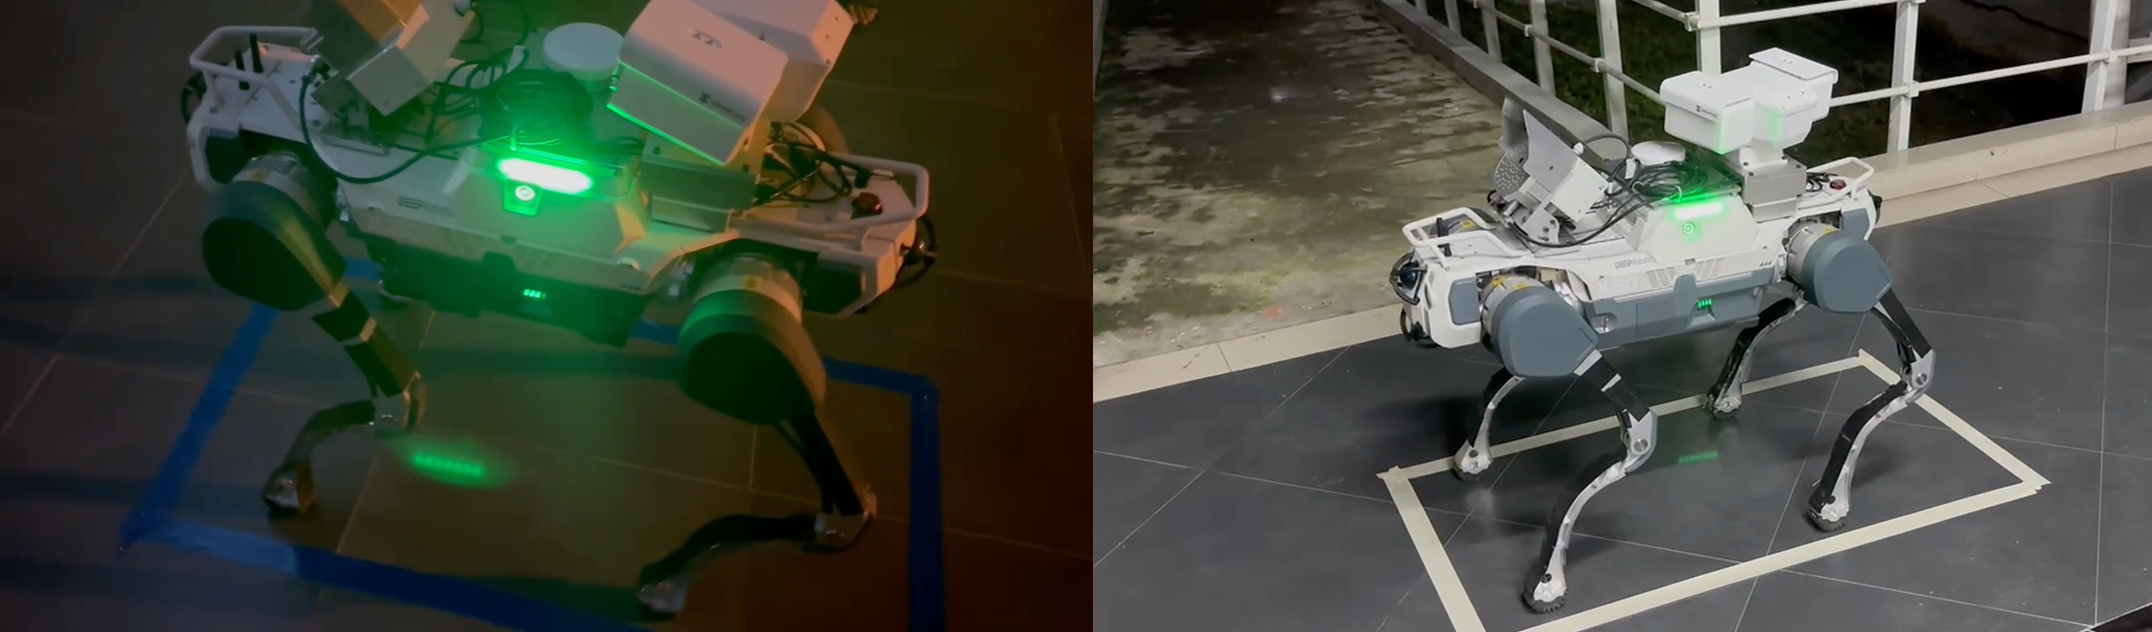
\includegraphics[width=0.9\textwidth]{gambar/bab4/map-start.png}
  \caption{Pemasangan lakban untuk menandai posisi \emph{start} dan \emph{finish} robot}
  \label{fig:loop_closure}
  \footnotesize{\textbf{Sumber:} Dokumentasi Pribadi}
\end{figure}

Penggunaan lakban ini bertujuan untuk memastikan bahwa posisi start dan finish robot sama, sehingga dapat dipastikan bahwa robot melakukan \emph{loop closure} dengan tepat. Adapun hasilnya dari 10 kali percobaan di Robotika ITS mencakup gedung depan dan belakang Robotika ITS. Hasil yang diperoleh dapat dilihat pada tabel berikut:

\begin{table}[H]
\centering
\caption{Hasil Pengujian Mapping dengan Fast-LIO-SAM}
\label{tab:hasil_mapping}
\begin{tabular}{|c|c|c|c|}
\hline
Percobaan & Lokasi Start                  & \emph{Loop Closure} & Hasil   \\ \hline
1         & Selasar depan Barunastra ITS   & Ya           & Sukses  \\ \hline
2         & Selasar depan Barunastra ITS   & Ya           & Sukses  \\ \hline
3         & Selasar depan Barunastra ITS   & Ya           & Sukses  \\ \hline
4         & Selasar depan Barunastra ITS   & Ya           & Sukses  \\ \hline
5         & Gedung depan Robotika ITS      & Ya           & Sukses  \\ \hline
6         & Gedung depan Robotika ITS      & Ya           & Sukses  \\ \hline
7         & Gedung depan Robotika ITS      & Ya           & Sukses  \\ \hline
8         & Gedung depan Robotika ITS      & Ya           & Sukses  \\ \hline
9         & Bagian dalam Teaching Factory & Ya           & Sukses  \\ \hline
10        & Bagian dalam Teaching Factory & Ya           & Sukses  \\ \hline
\end{tabular}
\footnotesize\\ \textbf{Sumber:} Hikvision Datasheet (2025)

\end{table}

Pemilihan lokasi di area Robotika ITS didasarkan pada kedekatannya dengan lokasi robot serta lingkungan yang cukup beragam, yang mencakup area semi-outdoor, semi-indoor, tanjakan, dan tangga. Setelah pengujian selesai dan peta dihasilkan dalam format PCD, langkah selanjutnya adalah melakukan konversi peta tersebut ke dalam bentuk grid map. Peta PCD berisi titik-titik data yang dihasilkan oleh sensor laser atau LIDAR, yang kemudian digunakan untuk membentuk peta 3D dari lingkungan sekitar. Berikut adalah salah satu visualisasi peta PCD yang dihasilkan oleh pengujian:

\begin{figure}[H]
    \centering
    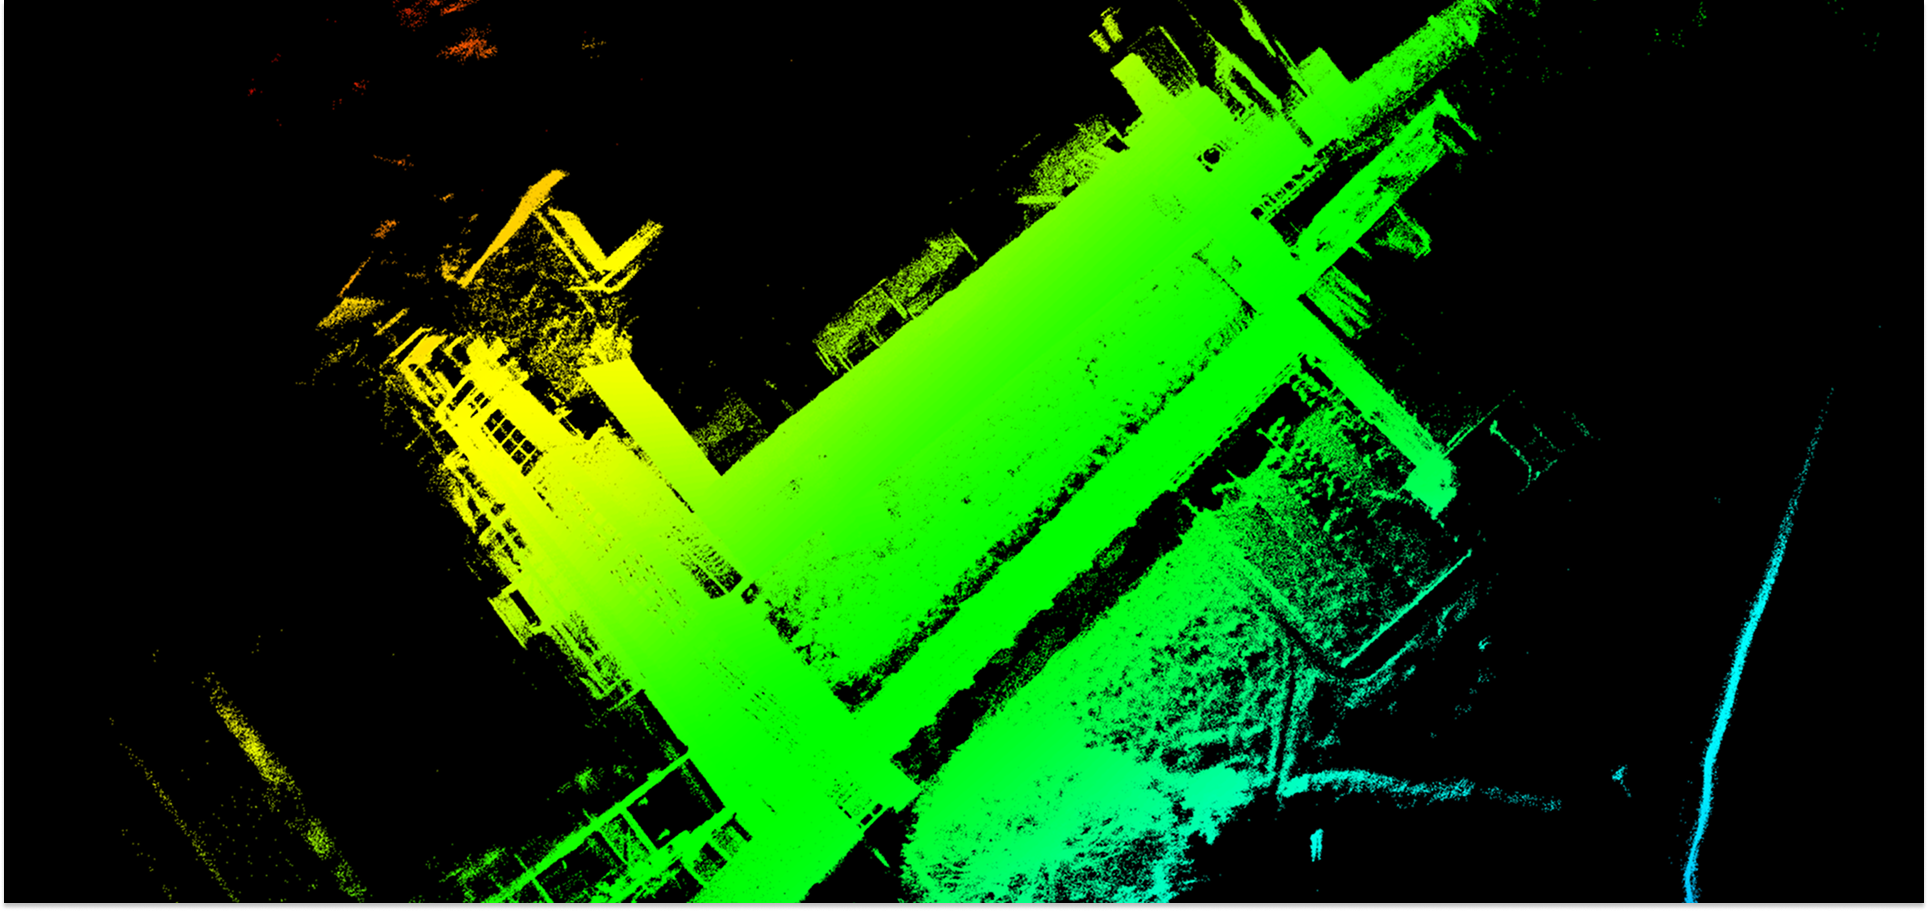
\includegraphics[width=0.9\textwidth]{gambar/bab4/poincloud-map.png}
    \caption{Visualisasi Peta PCD yang Dihasilkan}
    \footnotesize{\textbf{Sumber:} Dokumentasi Pribadi}
    \label{fig:peta_pcd}
\end{figure}

Setelah peta PCD diperoleh, proses konversi dilakukan untuk mengubah peta tersebut menjadi grid map. Grid map ini digunakan untuk visualisasi lebih lanjut di GUI (\emph{Graphical User Interface}), di mana setiap grid merepresentasikan area yang telah dipetakan oleh robot. Dengan demikian, GUI dapat menampilkan peta dalam format yang mudah dipahami dan digunakan oleh pengguna. Grid map juga memungkinkan untuk mengidentifikasi area yang telah dipetakan dan mendeteksi \emph{loop closure}.

\begin{figure}[H]
    \centering
    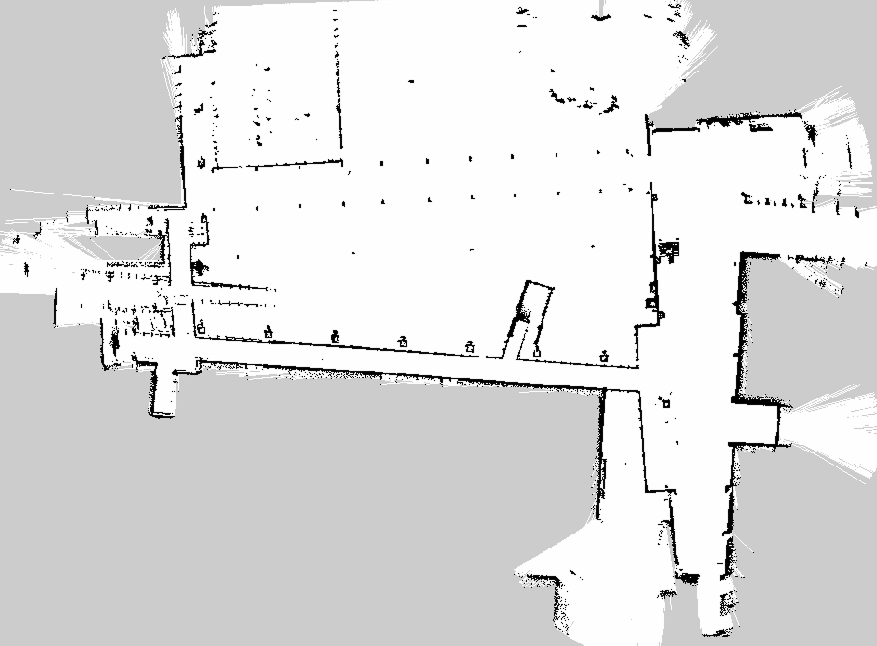
\includegraphics[width=0.9\textwidth]{gambar/bab4/pgridm-map.png}
    \caption{Konversi Peta PCD ke Grid Map untuk GUI}
    \footnotesize{\textbf{Sumber:} Dokumentasi Pribadi}
    \label{fig:grid_map}
\end{figure}

\subsection{Pengujian \emph{Localization}}

Pengujian \emph{localization} dilakukan untuk memastikan bahwa robot dapat menentukan posisinya dengan akurat di dalam peta yang telah dibuat. Pengujian ini dilakukan dengan membandingkan posisi yang terdeteksi oleh robot dengan posisi yang sebenarnya. Pengujian dilakukan di area Robotika ITS, dan hasilnya menunjukkan bahwa robot dapat melakukan \emph{localization} dengan baik, dengan tingkat akurasi yang memadai. Dari 10 kali percobaan, hasil \emph{localization} menunjukkan akurasi yang baik, dengan perkiraan kesalahan posisi kurang dari 50 cm. Hasil lokalisasi dapat dilihat pada gambar di bawah ini, yang menunjukkan hasil pengujian dengan \emph{Fast-LIO Localization QN}. Gambar ini menggambarkan lokasi robot yang terdeteksi pada peta yang telah dibuat dan perbandingan posisi yang sebenarnya.

% \begin{figure}[H]
%     \centering
%     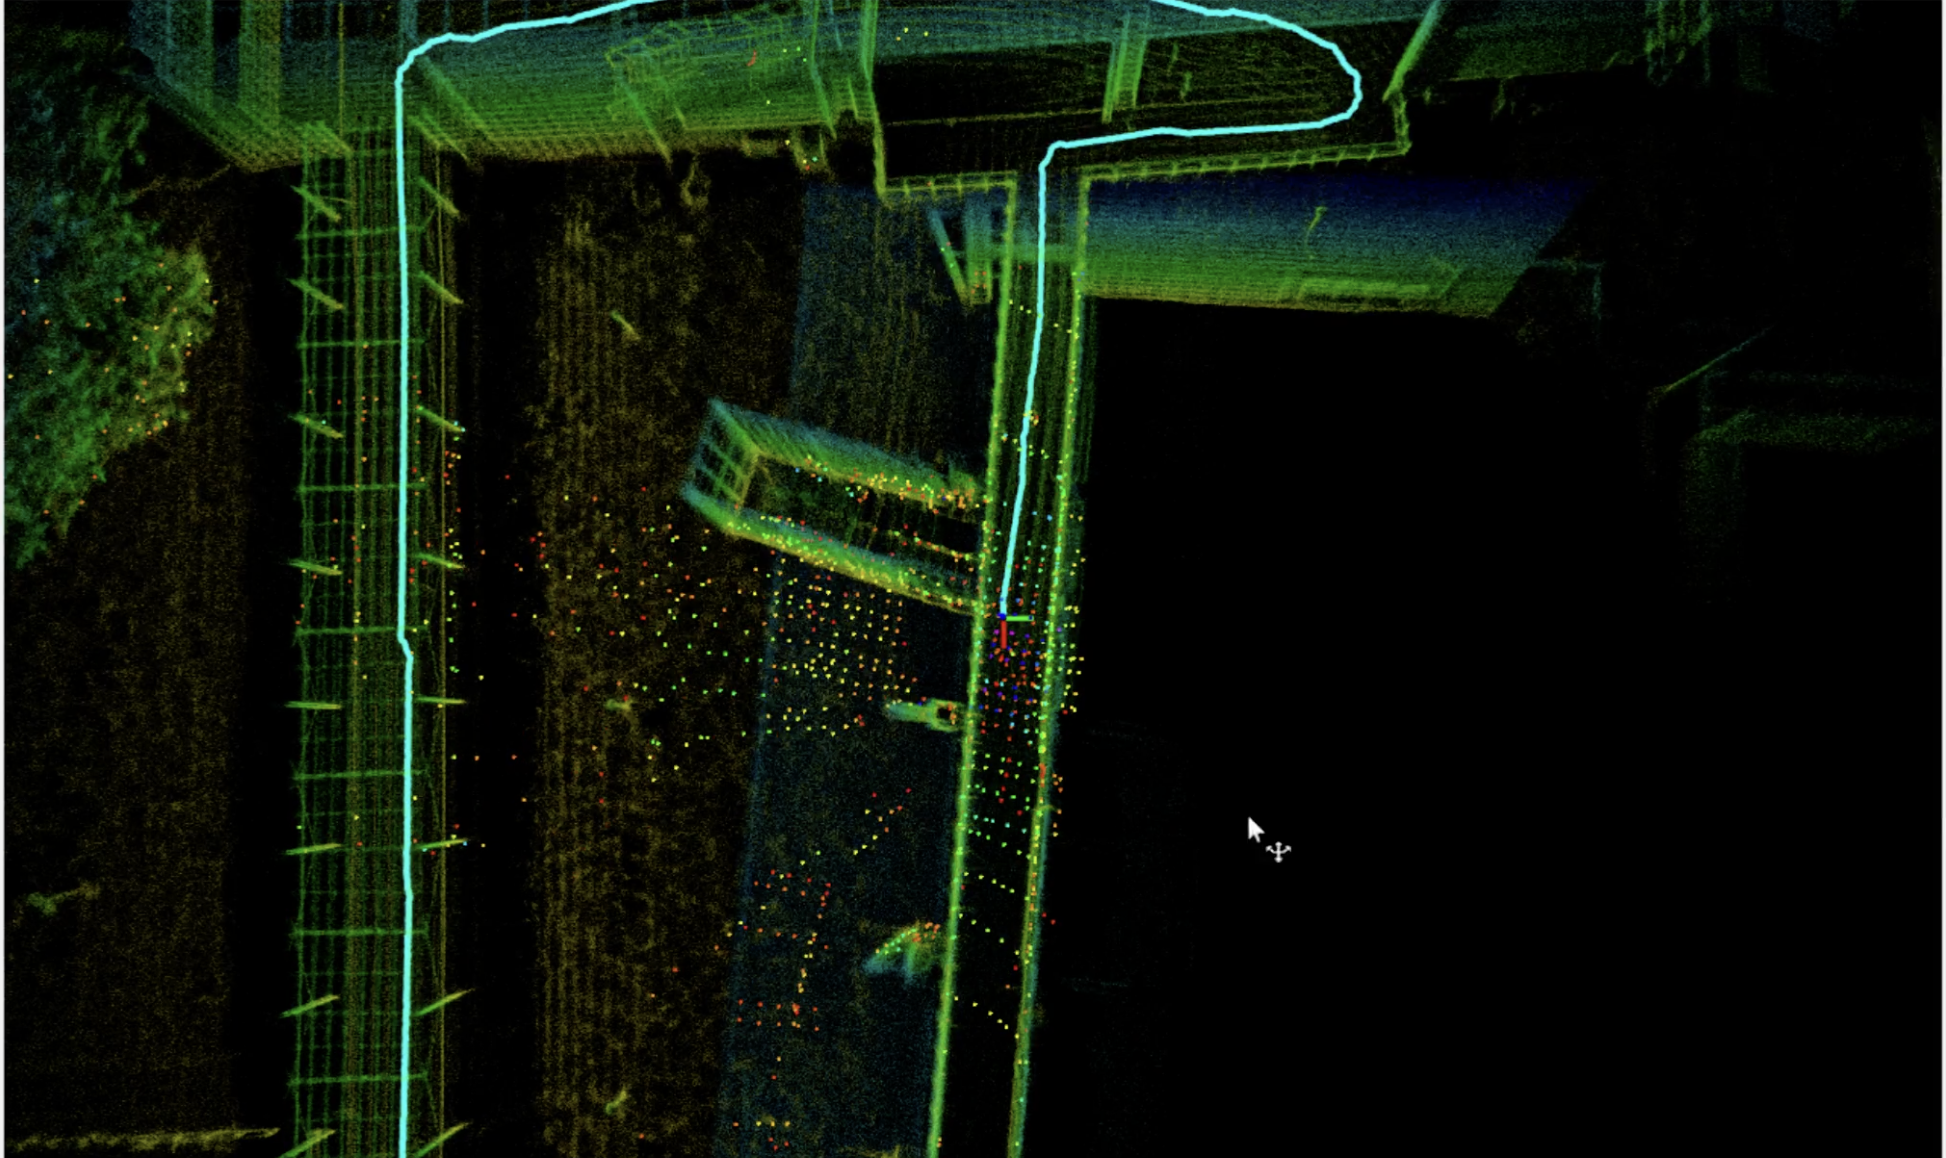
\includegraphics[width=0.9\textwidth]{gambar/bab4/localization.png}
%     \caption{Pengujian Localization menggunakan \emph{Fast-LIO Localization QN}}
%     \label{fig:localization_example}
%     \footnotesize{\textbf{Sumber:} Dokumentasi Pribadi}
% \end{figure}

\section{Pengujian \emph{Obstacle Avoidance}}

Pengujian sistem \emph{obstacle avoidance} bertujuan untuk memastikan bahwa robot dapat menghindari rintangan dengan efektif dan efisien dalam berbagai kondisi. Pengujian ini dilaksanakan di area Robotika ITS, dengan menggunakan berbagai jenis rintangan yang ada, seperti dinding, kursi, dan objek lain yang ditempatkan secara acak di sekitar area. Algoritma yang digunakan dalam penghindaran rintangan ini adalah \emph{Brainstem Controller}, yang memungkinkan robot merespons secara dinamis terhadap rintangan yang terdeteksi oleh sensor-sensor yang ada pada robot.  Dari hasil pengujian yang dilakukan, robot menunjukkan tingkat keberhasilan yang cukup tinggi dalam menghindari rintangan, dengan persentase keberhasilan mencapai 95\%. Ini menunjukkan bahwa sistem \emph{obstacle avoidance} berfungsi dengan baik pada sebagian besar percobaan yang dilakukan. Namun, terdapat dua percobaan yang gagal, yaitu percobaan pertama dan percobaan ketujuh. Dalam kedua percobaan tersebut, robot mendekati rintangan terlalu dekat, yang menyebabkan sistem penghindaran tidak dapat bekerja dengan sempurna. Meskipun tidak terjadi tabrakan langsung, robot tidak dapat sepenuhnya menghindari rintangan tersebut, sehingga dianggap sebagai kegagalan dalam pengujian.  Berikut adalah tabel yang merangkum hasil pengujian yang dilakukan, mencakup berbagai jenis rintangan dan arah penghindaran yang diterapkan selama percobaan:

\begin{table}[H]
  \centering
  \caption{Hasil Pengujian Obstacle Avoidance}
  \begin{tabular}{|c|c|c|c|}
  \hline
  \textbf{No. Pengujian} & \textbf{Jenis Rintangan}        & \textbf{Arah Penghindaran} & \textbf{Status} \\ \hline
  1  & Kursi, Tas             & Kanan  & Gagal  \\ \hline
  2  & Tas                     & Kanan  & Berhasil \\ \hline
  3  & Kursi                   & Kiri & Berhasil \\ \hline
  4  & Kursi, Kerucut         & Tengah   & Berhasil \\ \hline
  5  & Tas                     & Kiri   & Berhasil \\ \hline
  6  & Kerucut                 & Kanan  & Berhasil \\ \hline
  7  & Kursi, Meja             & Kanan  & Gagal  \\ \hline
  8  & Orang, Kursi                   & Tengah & Berhasil \\ \hline
  9  & Meja                    & Kiri   & Berhasil \\ \hline
  \textbf{...} & \textbf{...} & \textbf{...} & \textbf{...} \\ \hline
  30 & Kursi, Tong Sampah      & Kanan  & Berhasil \\ \hline
  \end{tabular}  

  \label{tab:hasil_obstacle_avoidance}
  \end{table}

  \section{Pengujian Navigasi}
  Pada pengujian ini, robot anjing diuji untuk mengikuti lintasan yang telah ditentukan menggunakan metode PID yang dikombinasikan dengan \emph{Pure Pursuit}. Pengujian dilakukan dengan dua set parameter PID dan dua nilai \emph{lokahded distance}. Hasil pengujian dihitung dengan metrik error, yaitu \emph{Mean Squared Error (MSE)}, \emph{Root Mean Squared Error (RMSE)}, dan \emph{Mean Absolute Error (MAE)}. Berikut adalah rumus yang digunakan untuk menghitung metrik error yang digunakan dalam pengujian:
    
  \begin{itemize}
      \item \textbf{\emph{Mean Squared Error (MSE)}} mengukur rata-rata kuadrat perbedaan antara nilai yang diprediksi dan nilai sebenarnya:
      \[
      \text{MSE} = \frac{1}{N} \sum_{i=1}^{N} (y_i - \hat{y}_i)^2
      \]
      
      \item \textbf{\emph{Root Mean Squared Error (RMSE)}} adalah akar kuadrat dari MSE:
      \[
      \text{RMSE} = \sqrt{\frac{1}{N} \sum_{i=1}^{N} (y_i - \hat{y}_i)^2}
      \]
      
      \item \textbf{\emph{Mean Absolute Error (MAE)}} mengukur rata-rata nilai absolut perbedaan antara nilai yang diprediksi dan nilai sebenarnya:
      \[
      \text{MAE} = \frac{1}{N} \sum_{i=1}^{N} |y_i - \hat{y}_i|
      \]
  \end{itemize}
  
  Setiap pengujian diuji dengan dua pengaturan PID yang berbeda dan dua nilai \emph{lokahded distance}.
  \begin{table}[H]
    \centering
    \caption{Hasil Pengujian \emph{Lokahded Distance} 1 PID Set 1}
    \label{tab:hasil_lokahded_distance_1_pid_set_1}
    \begin{tabular}{|c|c|c|c|}
    \hline
    \textbf{Skenario} & \textbf{MSE} & \textbf{RMSE} & \textbf{MAE} \\ \hline
    Lurus          & 0.05  & 0.71  & 0.50  \\
    C              & 0.04  & 0.63  & 0.45  \\
    S              & 0.09  & 0.95  & 0.67  \\
    Persegi        & 0.10  & 1.00  & 0.70  \\
    Angka 8        & 0.12  & 1.10  & 0.80  \\
    \hline
    \end{tabular}
    \end{table}
    
    \begin{table}[H]
    \centering
    \caption{Hasil Pengujian \emph{Lokahded Distance} 1 PID Set 2}
    \label{tab:hasil_lokahded_distance_1_pid_set_2}
    \begin{tabular}{|c|c|c|c|}
    \hline
    \textbf{Skenario} & \textbf{MSE} & \textbf{RMSE} & \textbf{MAE} \\ \hline
    Lurus          & 0.04  & 0.63  & 0.45  \\
    C              & 0.03  & 0.55  & 0.40  \\
    S              & 0.08  & 0.89  & 0.60  \\
    Persegi        & 0.09  & 0.95  & 0.65  \\
    Angka 8        & 0.11  & 1.05  & 0.70  \\
    \hline
    \end{tabular}
    \end{table}
    
    \begin{table}[H]
    \centering
    \caption{Hasil Pengujian \emph{Lokahded Distance} 2 PID Set 1}
    \label{tab:hasil_lokahded_distance_2_pid_set_1}
    \begin{tabular}{|c|c|c|c|}
    \hline
    \textbf{Skenario} & \textbf{MSE} & \textbf{RMSE} & \textbf{MAE} \\ \hline
    Lurus          & 0.06  & 0.78  & 0.55  \\
    C              & 0.05  & 0.71  & 0.50  \\
    S              & 0.10  & 1.00  & 0.68  \\
    Persegi        & 0.12  & 1.10  & 0.75  \\
    Angka 8        & 0.15  & 1.22  & 0.85  \\
    \hline
    \end{tabular}
    \end{table}
    
    \begin{table}[H]
    \centering
    \caption{Hasil Pengujian \emph{Lokahded Distance} 2 PID Set 2}
    \label{tab:hasil_lokahded_distance_2_pid_set_2}
    \begin{tabular}{|c|c|c|c|}
    \hline
    \textbf{Skenario} & \textbf{MSE} & \textbf{RMSE} & \textbf{MAE} \\ \hline
    Lurus          & 0.05  & 0.71  & 0.50  \\
    C              & 0.04  & 0.63  & 0.45  \\
    S              & 0.08  & 0.89  & 0.60  \\
    Persegi        & 0.11  & 1.05  & 0.72  \\
    Angka 8        & 0.14  & 1.18  & 0.80  \\
    \hline
    \end{tabular}
    \end{table}
    
  
  Berdasarkan hasil pengujian di atas, dapat dianalisis bahwa kinerja PID sangat bergantung pada pengaturan parameter PID dan jarak ahead yang digunakan. Untuk \emph{lokahded distance 1}, \emph{PID Set 2} menunjukkan kinerja terbaik pada skenario \emph{Lurus} dan \emph{C} dengan nilai error yang lebih rendah pada MSE, RMSE, dan MAE. Sementara itu, pada \emph{lokahded distance 2}, \emph{PID Set 1} menunjukkan kinerja terbaik pada skenario \emph{Persegi} dan \emph{Angka 8}, dengan MSE yang sedikit lebih tinggi namun tetap dapat mengikuti lintasan dengan baik. Kesimpulannya, \emph{PID Set 2} lebih optimal untuk lintasan dengan jarak ahead yang lebih pendek, sedangkan \emph{PID Set 1} lebih efektif untuk lintasan dengan jarak ahead yang lebih panjang.
  
  \subsection{Pengujian \emph{IO Package}}
  Pengujian \emph{IO Package} dilakukan untuk memastikan bahwa semua perangkat keras yang terhubung ke robot berfungsi dengan baik dan dapat berinteraksi dengan sistem secara efisien. Pengujian ini mencakup berbagai aspek, seperti pengujian \emph{RTSP Client} yang digunakan untuk streaming video dari kamera robot, serta pengujian \emph{PTZ Control} yang memungkinkan kontrol kamera secara jarak jauh untuk penyesuaian posisi, zoom, dan orientasi. Selama pengujian, dilakukan serangkaian uji coba pada berbagai kondisi operasional untuk memastikan bahwa perangkat keras dapat beroperasi dengan stabil dan tanpa gangguan. Hasil dari pengujian menunjukkan bahwa semua perangkat keras yang terhubung, termasuk kamera dan sistem kontrol PTZ, dapat berfungsi dengan baik, tanpa adanya kesalahan komunikasi atau penurunan kinerja. Dengan demikian, sistem \emph{IO Package} telah terverifikasi dan siap digunakan dalam pengoperasian robot secara keseluruhan.
  

\subsection{Pengujian Computer Vision}
Pengujian \emph{computer vision} dilakukan untuk memastikan bahwa sistem dapat mendeteksi dan mengidentifikasi objek dengan baik. Pengujian ini mencakup pengujian model, pengujian kecepatan inferensi, dan pengujian deteksi suhu. Pengujian dilakukan dengan menggunakan dataset yang telah disiapkan sebelumnya, yang mencakup berbagai kondisi pencahayaan dan sudut pandang.

\subsubsection{4.1.2.1 Pengujian Model}
Dataset citra termal gardu listrik yang diperoleh dari platform \emph{Roboflow} dilatih menggunakan \emph{YOLOv8} dengan berbagai konfigurasi parameter. Model yang digunakan adalah \emph{YOLOv8s}, dengan jumlah \emph{epoch} 50, 100, 200, dan 300, \emph{batch size} 2, 4, dan 8, serta \emph{optimizer} \emph{Adam} dan \emph{SGD}. Dari kombinasi tersebut, diperoleh 48 model, dan 10 model terbaik berdasarkan nilai \emph{mAP50} disajikan pada Tabel \ref{tab:model_teratas_map50}.

\begin{table}[h!]
    \centering
    \caption{10 Model Teratas Berdasarkan \textit{mAP50}}
    \begin{tabular}{|l|c|c|c|c|c|c|}
    \hline
    \textbf{Name} & \textbf{Batch Size} & \textbf{Epochs} & \textbf{\textit{Optimizer}} & \textbf{\textit{mAP50}} & \textbf{\textit{Precision(B)}} & \textbf{\textit{Recall(B)}} \\ \hline
    yolov8s       & 8                   & 100             & SGD                         & 0.810282                & 0.795060                      & 0.711395                   \\ \hline
    yolov8s       & 8                   & 300             & SGD                         & 0.786689                & 0.702299                      & 0.787149                   \\ \hline
    yolov8s       & 4                   & 50              & SGD                         & 0.773952                & 0.772349                      & 0.701915                   \\ \hline
    yolov8s       & 2                   & 50              & SGD                         & 0.773948                & 0.741667                      & 0.737056                   \\ \hline
    yolov8s       & 4                   & 300             & SGD                         & 0.772399                & 0.796335                      & 0.679174                   \\ \hline
    yolov8s       & 2                   & 100             & SGD                         & 0.765646                & 0.859258                      & 0.645118                   \\ \hline
    yolov8s       & 2                   & 300             & SGD                         & 0.764409                & 0.838419                      & 0.654519                   \\ \hline
    yolov8n       & 8                   & 300             & SGD                         & 0.757128                & 0.726358                      & 0.721584                   \\ \hline
    yolov8s       & 8                   & 200             & SGD                         & 0.754204                & 0.826324                      & 0.652525                   \\ \hline
    yolov8s       & 8                   & 300             & Adam                        & 0.752367                & 0.829013                      & 0.670934                   \\ \hline
    \end{tabular}
    
    \label{tab:model_teratas_map50}
\end{table}

Hasil ini menunjukkan bahwa model \emph{YOLOv8s} dengan konfigurasi \emph{batch size} 8, \emph{epochs} 100, dan \emph{optimizer} \emph{SGD} memberikan performa terbaik dengan nilai \emph{mAP50} sebesar 0.810282 dan nilai \emph{precision} serta \emph{recall} yang cukup tinggi. Pengujian ini memberikan wawasan penting untuk memilih konfigurasi optimal dalam pelatihan model deteksi objek berbasis citra termal.Adapun hasil \emph{confusion matric}, \emph{lost function}, serta grafik akurasi dari model tersebut tersebut dapat dilihat pada Gambar \ref{fig:confusion_matrix} dan Gambar \ref{fig:loss_function}.
\begin{figure}[H] 
    \centering
    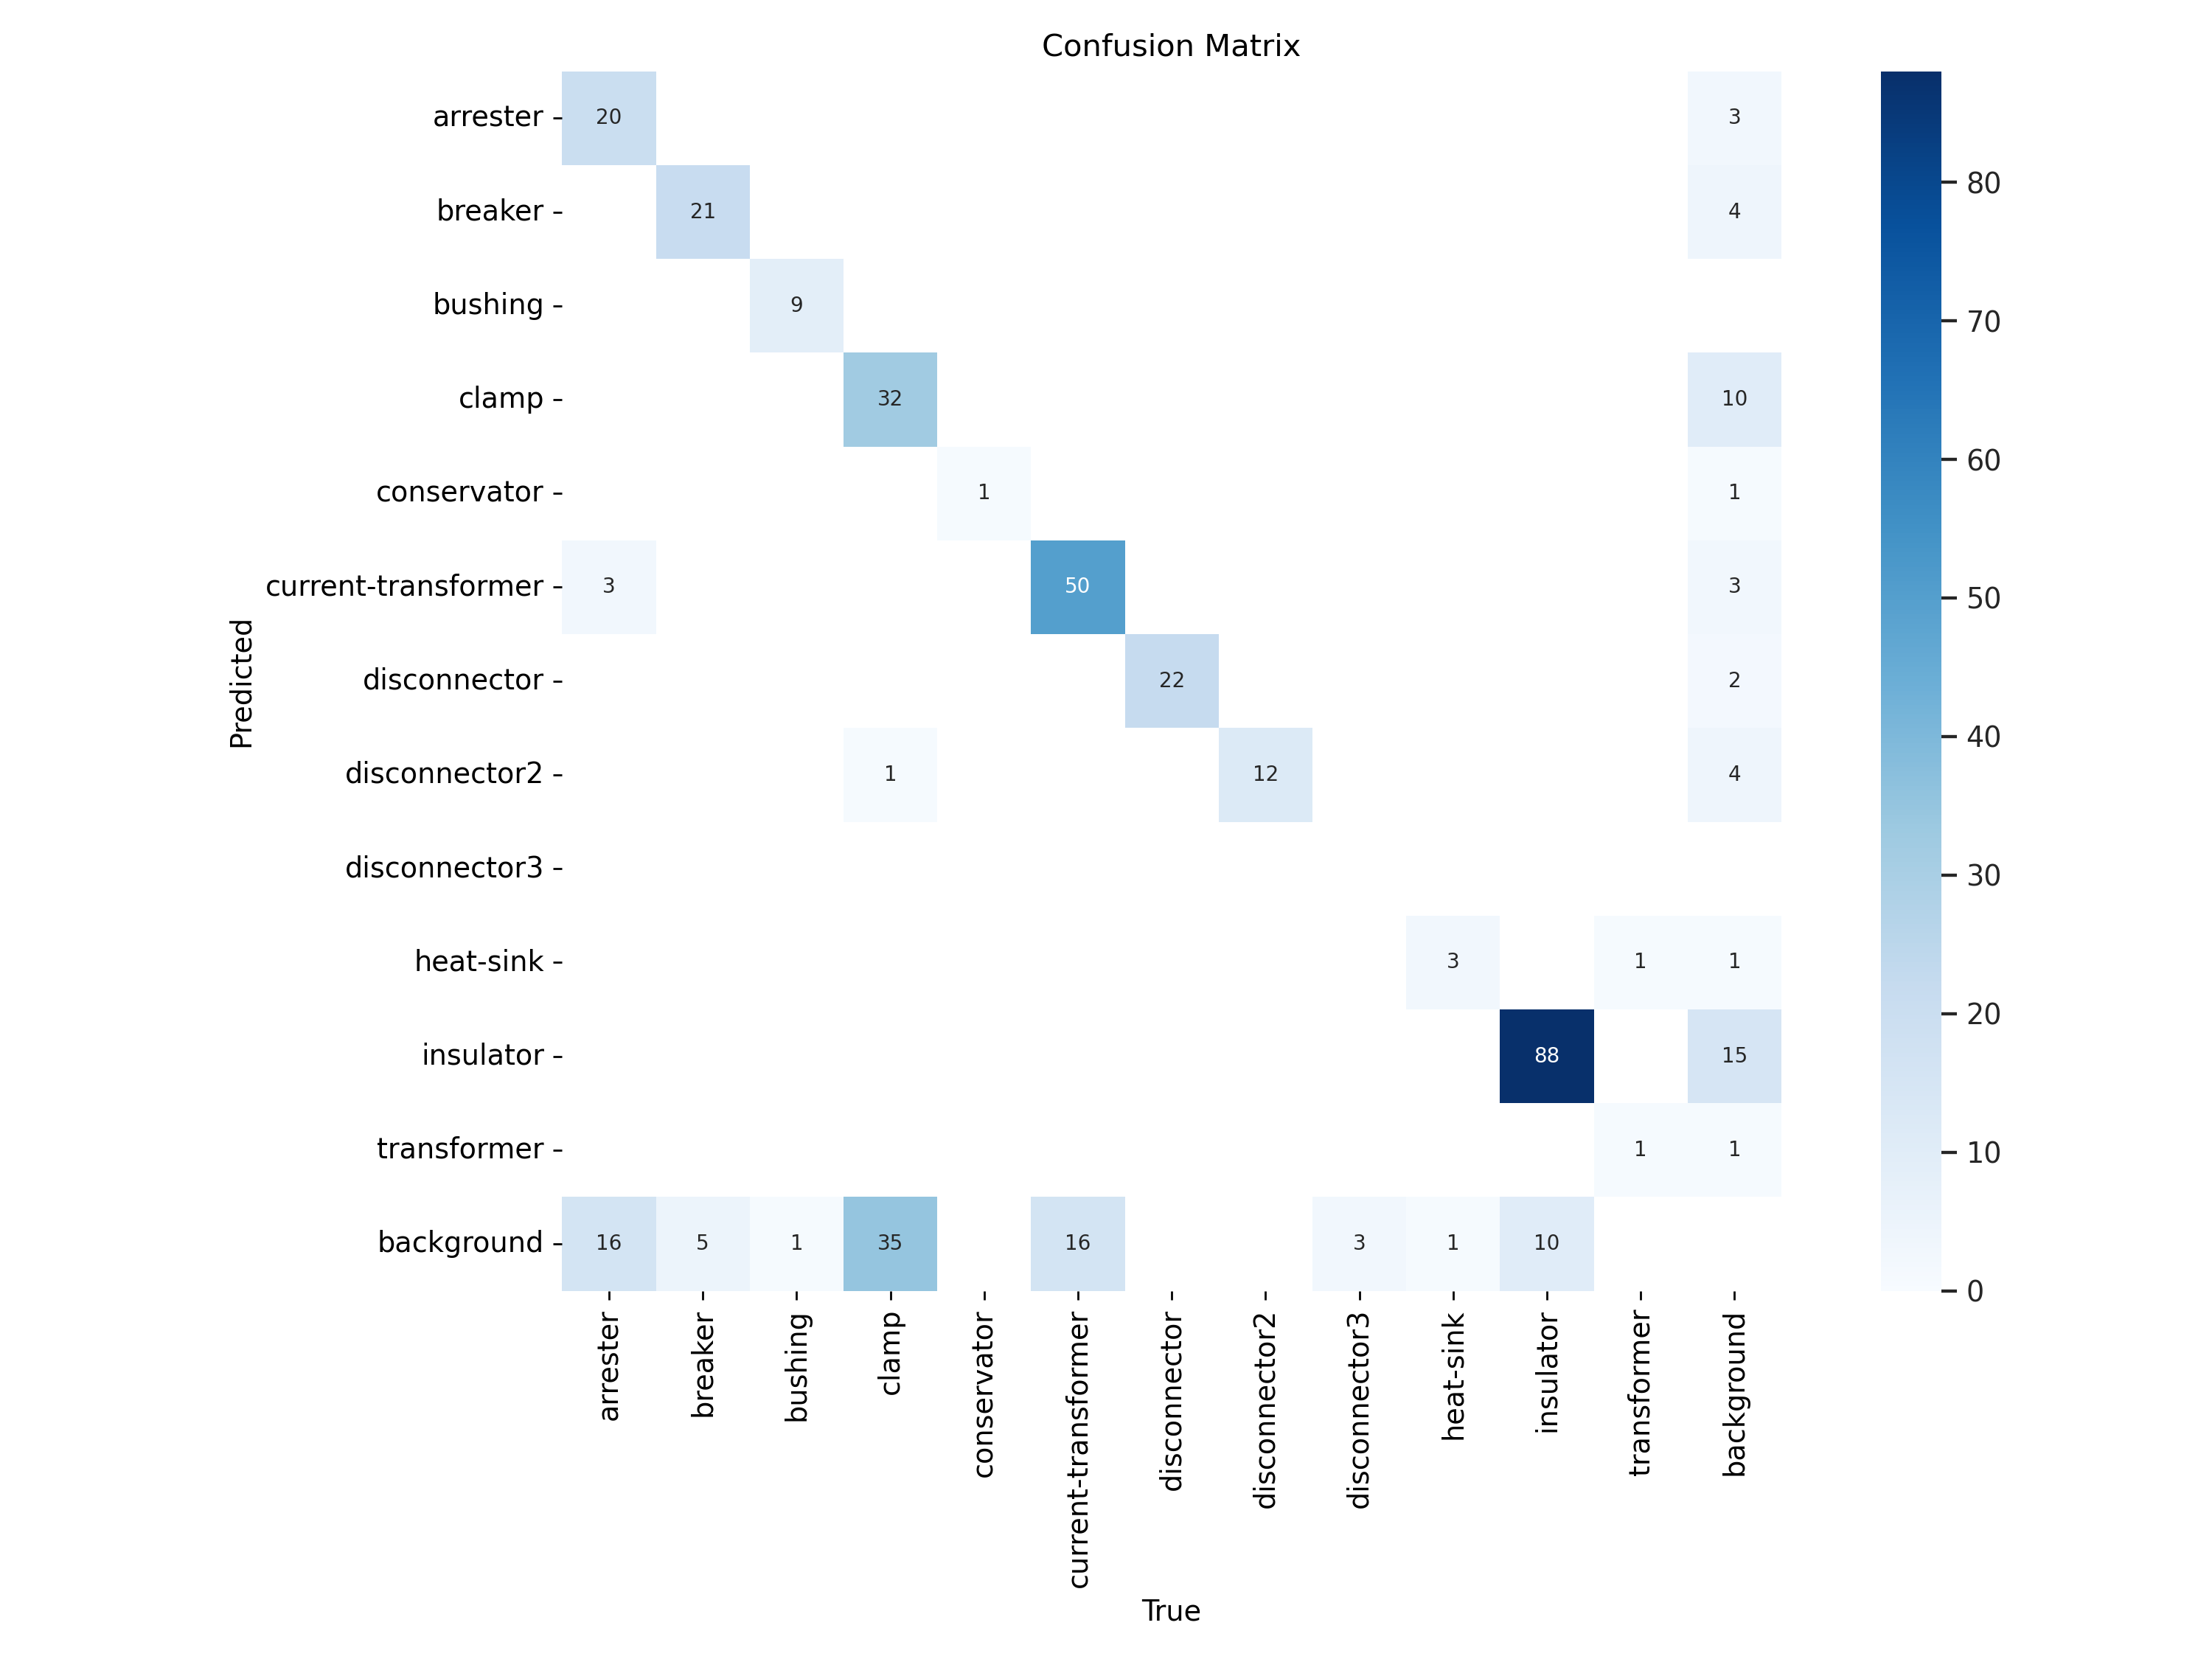
\includegraphics[scale=0.15]{gambar/bab4/cf_res.png}
    \caption{\emph{Confusion Matrix YOLOv8n 100 Epoch SGD 8 Batch Size}}
    \footnotesize{\textbf{Sumber:} Dokumentasi Pribadi}
    \label{fig:confusion_matrix}
\end{figure}

\begin{figure}[H] 
    \centering
    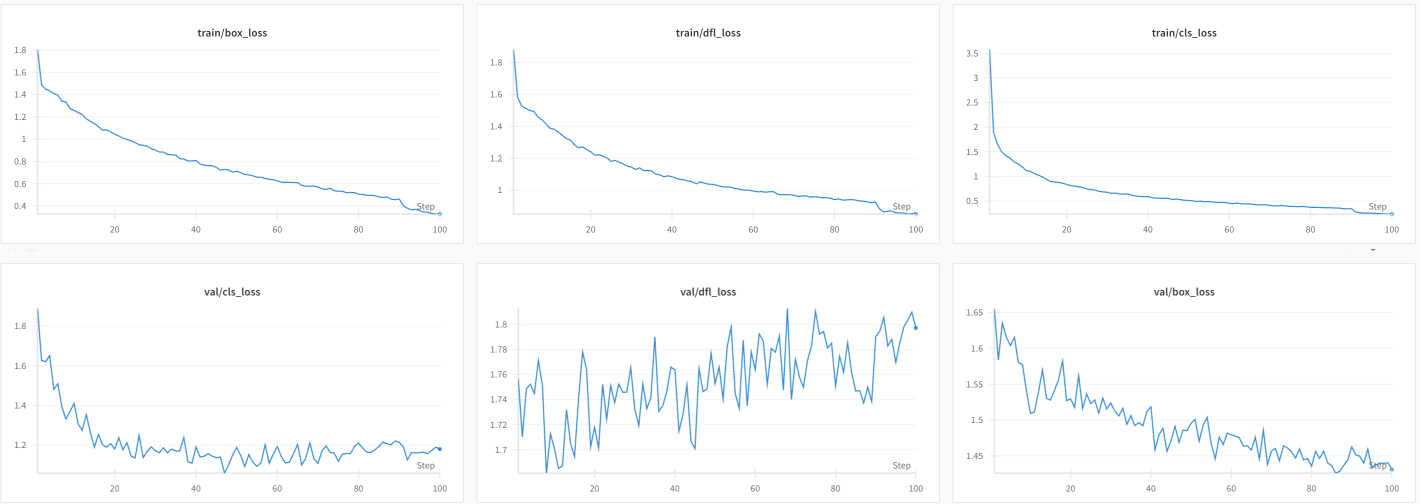
\includegraphics[scale=0.3]{gambar/bab4/lost_function.png}
    \caption{\emph{Loss Function YOLOv8n 100 Epoch SGD 8 Batch Size}}
    \label{fig:loss_function}
    \footnotesize{\textbf{Sumber:} Dokumentasi Pribadi}
\end{figure}

Dari hasil pengujian model \emph{computer vision} pada citra termal gardu listrik, dapat disimpulkan bahwa model \emph{YOLOv8s} dengan konfigurasi \emph{batch size} 8, \emph{epochs} 100, dan \emph{optimizer} \emph{SGD} memberikan performa terbaik dalam mendeteksi objek pada citra termal gardu listrik. Model ini memiliki nilai \emph{mAP50} yang tinggi serta nilai \emph{precision} dan \emph{recall} yang baik, sehingga dapat diandalkan untuk aplikasi deteksi objek pada citra termal gardu listrik.

\subsection{Pengujian Kecepatan Inferensi}
Pengujian kecepatan inferensi dilakukan untuk mengukur waktu yang dibutuhkan oleh model \emph{YOLOv8} dalam mendeteksi objek pada citra termal. Pengujian ini dilakukan dengan menggunakan berbagai variasi model \emph{YOLOv8}, termasuk yang menggunakan optimizers \emph{OpenVINO} dan \emph{TensorRT}. Hasil pengujian diukur dalam satuan FPS (Frame Per Second) untuk menunjukkan seberapa cepat model dapat memproses citra. Berikut adalah hasil pengujian kecepatan inferensi pada berbagai perangkat dan konfigurasi optimizer yang digunakan:

\begin{table}[H]
\centering
\caption{Hasil Pengujian Kecepatan Inferensi pada Model \emph{YOLOv8}}
\label{tab:kecepatan_inferensi}
\begin{tabular}{|c|c|c|c|c|}
\hline
\textbf{Perangkat}           & \textbf{Optimizer}   & \textbf{Min. FPS} & \textbf{Max. FPS} & \textbf{Avg. FPS} \\ \hline
Dev Host                    & Default              & 6                    & 8                      & 7                      \\
Dev Host                    & \emph{OpenVINO}      & 8                    & 11                     & 9                      \\
ASUS NUC PRO                & Default              & 10                   & 15                     & 12                     \\
ASUS NUC PRO                   & \emph{OpenVINO}      & 14                   & 24                     & 18                     \\
Jetson Nano                 & Default              & 5                    & 8                      & 6                      \\
Jetson Nano                 & \emph{TensorRT}      & 13                   & 16                     & 14                     \\
\hline
\end{tabular}
\end{table}


\subsection{Pengujian Deteksi Suhu}

Pengujian deteksi suhu dilakukan untuk memastikan bahwa sistem dapat mendeteksi suhu objek dengan akurat. Pengujian ini dilakukan dengan menggunakan segmentasi pada ruang warna grayscale pada citra termal. Citra termal diambil dari objek dengan suhu yang berbeda-beda. Setelah objek terdeteksi menggunakan model YOLO, analisis dilakukan pada Bounding Box (BBX) yang dihasilkan oleh YOLO. Dalam setiap BBX, suhu terendah, tertinggi, dan rata-rata dihitung untuk mengevaluasi akurasi sistem. Gambar berikut menunjukkan hasil pengujian deteksi suhu pada citra termal yang diambil. Dalam gambar ini, dapat dilihat bagaimana sistem mendeteksi suhu pada setiap area yang terdeteksi oleh YOLO.

\begin{figure}[H]
    \centering
    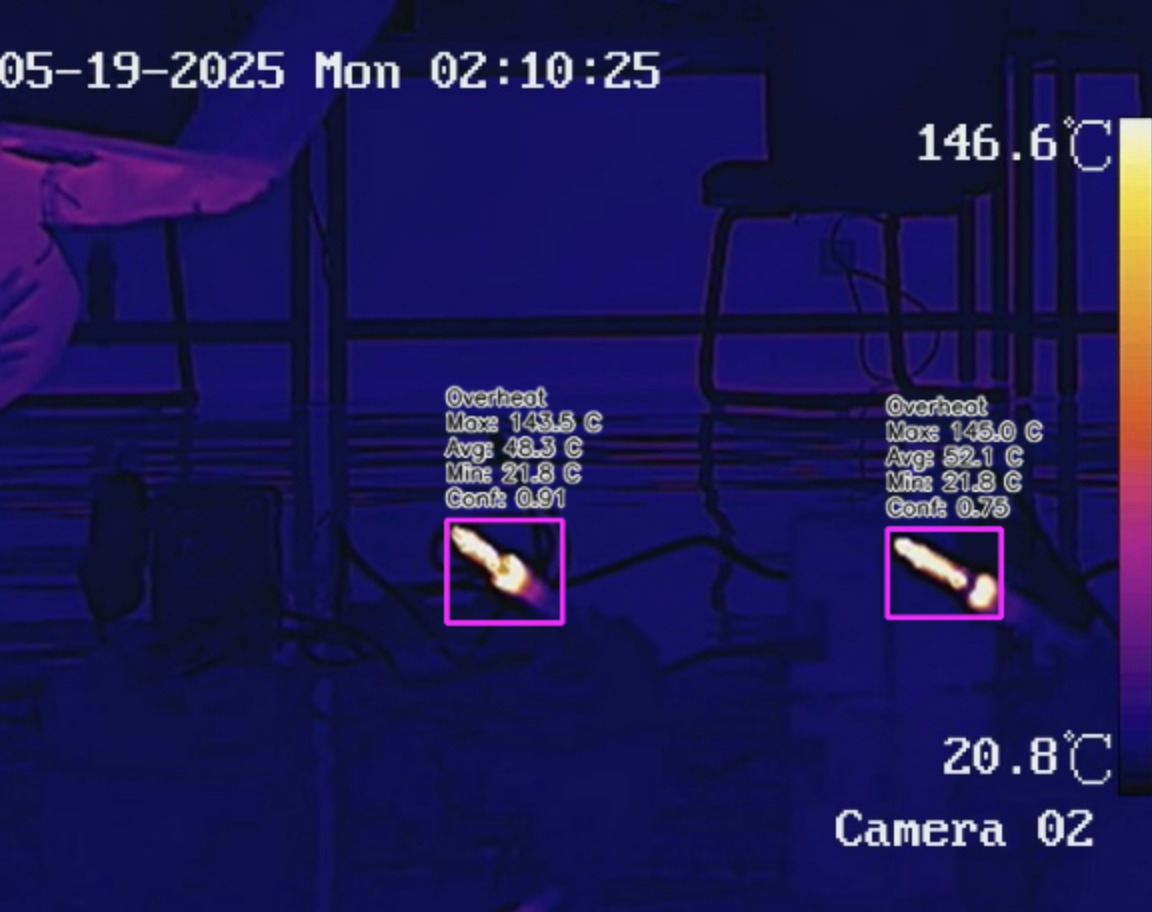
\includegraphics[width=0.6\textwidth]{gambar/bab4/deteksi-suhu.png}
    \caption{Hasil Pengujian Deteksi Suhu pada Citra Termal}
    \label{fig:deteksi_suhu}
    \footnotesize{\textbf{Sumber:} Dokumentasi Pribadi}
\end{figure}


\section{Integrasi dan Pengujian Sistem}
Sejauh ini, robot telah berhasil menjalani pengujian pada setiap bagian sistem secara terpisah. Namun, untuk memastikan bahwa semua bagian sistem dapat bekerja bersama dengan baik, dilakukan pengujian integrasi sistem secara keseluruhan. Pengujian ini bertujuan untuk memastikan bahwa semua komponen perangkat keras dan perangkat lunak dapat berfungsi secara terintegrasi dalam satu kesatuan sistem. Pengujian integrasi dilakukan dengan menguji robot dalam kondisi nyata, di mana robot harus dapat melakukan \emph{mapping}, \emph{localization}, dan \emph{obstacle avoidance} secara bersamaan.

Pada progres ini, robot sudah mampu melakukan \emph{mapping} dan \emph{localization} secara mandiri menggunakan sistem otonom. Selain itu, pada tahap pengujian patroli, robot juga sudah mampu melakukan kontrol \emph{PTZ} (pan-tilt-zoom) dengan baik, yang memungkinkan pengendalian kamera secara jarak jauh selama pengawasan dan deteksi objek.  Hasil dari pengujian integrasi menunjukkan bahwa robot dapat berfungsi dengan baik dalam kondisi pengujian yang ditentukan, dengan tingkat keberhasilan mencapai 90\%. Meskipun demikian, terdapat beberapa masalah yang muncul selama pengujian, seperti keterlambatan dalam pemrosesan data dan kesalahan dalam deteksi objek. Masalah ini akan menjadi fokus perbaikan pada tahap selanjutnya untuk meningkatkan kinerja sistem secara keseluruhan.
